% !TeX spellcheck = en_GB
\label{chapter:experiments}

	In this chapter we are going to explain the final models we chose for our work and the input data preparation to feed these models with. For the different solutions, we have used the algorithms previously explained in the methodology section \ref{section:models}. Below, a list including the 6 implementations compared follows:
	
	\begin{itemize}
		\item \acrshort{svm} classifier for multiclass classification
		\item \acrshort{svm} multiclass + \acrshort{svm} for a final binary classification
		\item \acrshort{lstm} for multiclass classification
		\item \acrshort{lstm} multiclass + \acrshort{svm} for a final binary classification
		\item \acrshort{cnn} for multiclass classification
		\item \acrshort{cnn} multiclass + \acrshort{svm} for a final binary classification
	\end{itemize}
	

\section{Input data preparation}
\label{section:input-data-preparation}

	For the proposed experiments, we have decided to build a small dataset with the embeddings extracted form the .\textit{tfrecord} files that belong to 14 classes: half of them \textit{violent} and the other half, \textit{non-violent}. To find these, we first did a run on the simple user-interaction program that is explained in \ref{subsection:violent-classes} as if we were gender-based violence victims. As we said a total of 28 classes were selected. From this set, we picked 7 as the violent classes. The other 7 were chosen just by looking at the ontology to provide negative classes.
	
	It is important to mention that this collection of data is composed by samples with just one label assigned. As explained before in \ref{section:audioset}, the Audio Set database is highly unbalanced. Some of the most appropriated classes to be considered violence are scarcely populated. When doing the selection of categories, apart from paying attention to the own meaning of the class, we also checked the number of samples. For the non-violent type, this was not a problem, since we took some of the most populated labels. However, in the violent case, we had to deal with the requirement of representing violence and also having enough observations. So, due to these limitations, we could not obtain a naturally balanced set. In table \ref{table:7}, the 14 selected labels are shown. %that were selected divided in violent and non-violent. 
	In figure \ref{fig:mesh14}, a bar plot shows the number of samples obtained per class right after the selection. 
	
	\begin{table}[ht]
		\centering
		\begin{tabular}{|| m{10em} | m{10em} ||}
			\hline
			\textbf{Violent} & \textbf{Non-violent} \\
			\hline\hline
			Baby cry, infant cry & Printer \\
			\hline
			Slap, smack & Music \\
			\hline
			Screaming & Speech \\
			\hline
			Machine gun & Vehicle \\
			\hline
			Breaking & Animal \\
			\hline
			Slam & Dishes, pots, and pans \\
			\hline
			Yell & Wind \\
			\hline
		\end{tabular}
	\caption{Relation of \textit{violent} and \textit{non-violent} selected classes}
	\label{table:7}
	\end{table}
	
	\begin{figure}[t]
		\centering
		\captionsetup{justification=centering}
		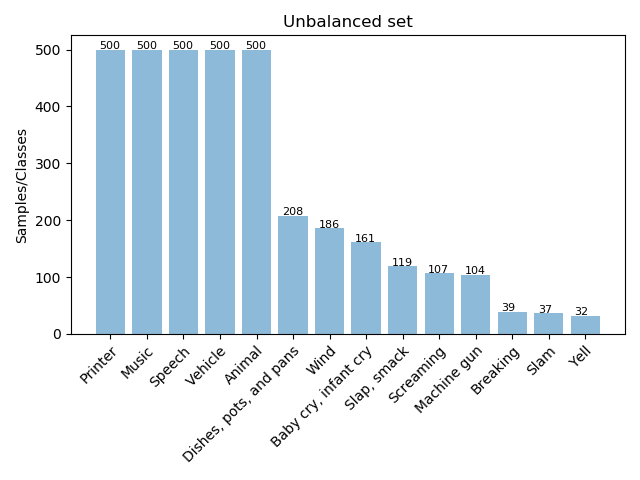
\includegraphics[scale=0.6]{samples-class-experiments}
		\caption{Bar plot that shows the number of samples for each of the selected classes. Clearly, the violent categories are much less populated than the others, that did not have to much any semantic criteria}
		\label{fig:mesh14}
	\end{figure}

	Some initial preprocessing steps were performed before passing the data to the different models. As mentioned in \ref{subsection:extracting-embeddings}, we had to deal with the zero-filling problem, which means that some of the rows of the embeddings matrices are completely zero because the duration of the original video is less than 10s. As a solution, we decided to substitute the zero numbers in all the data with the machine epsilon\footnote{The machine epsilon value is considered the smallest value that satisfies $1 + \epsilon_{match} > 1$. It is the difference between one and the next closest number that is representable as a machine value \cite{Kaw}} value. 
	
	However, in the two models that use \acrshort{svm} for the multiclass classification a different solution was proposed. As it was explained in subsection \ref{label:svm}, this algorithm needs the input data matrix to be in the form [$number\ of\ samples\ \times\ number\ of\ features$], which differs from the originally shape of our data, [$number\ of\ samples\ \times\ number\ of\ seconds\ \times\ number\ of\ features$]. For this reason, we decided to reshape our data to the required form which resulted in a matrix of shape [$(number\ of\ samples\ \times\ number\ of\ seconds)\ \times\ number\ of\ features$]. With this conversion, instead of working  full audio instances, the data samples became the seconds of those instances. In order to remove zero data, we first checked the amount of zero-rows in every class. Since it was not a very significant portion of the data, we took them out of the dataset. 
	
	Once we had our data with all non-zero values, we needed to convert the imbalanced set to balanced one. First, for the classification task, we divided our data into train, validation and test subsets, using a 20\% for last one. Then, we decided to exclude half of the samples from the most populated classes from the train and validation sets %half of the samples from the most populated classes 
	\footnote{\textit{Speech}, \textit{Music}, \textit{Vehicle} and \textit{Animal}}. In figure \ref{fig:mesh15}, subfigure (a) shows the distribution of data per class in the dataset for the models that use \acrshort{svm} multiclass classifier. In subfigure (b), the distribution for the other four cases is shown. Then, we wanted to generate new data for those with less observations by applying the data augmentation technique \acrshort{smote}, explained in subsection \ref{subsection:smote}. \doubt{This technique deduces a distribution for the given observations and generate synthetic samples within the distribution of each class until even the most populated category. CPM: ¡qué raro! ¿por qué iba a generar de la clase más poblada si esta es la que se toma como tope? No sé...}. Just the train and validation sets were subjected to this conversion process, leaving the test set with the original number of embeddings in their natural a priori distribution. The final shape of the input data for each of the experiments is shown in table \ref{table:8}.
	
	\begin{figure}[ht]
		% Whole figure
		\captionsetup{justification=centering}
		\begin{subfigure}[b]{\textwidth}
			% Start with figure wav
			\centering
			\captionsetup{justification=centering}
			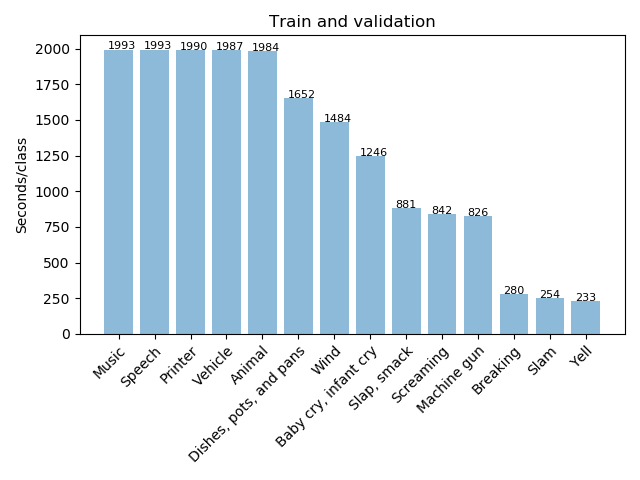
\includegraphics[width=0.5\linewidth]{tr_val_unbal_svm}%
			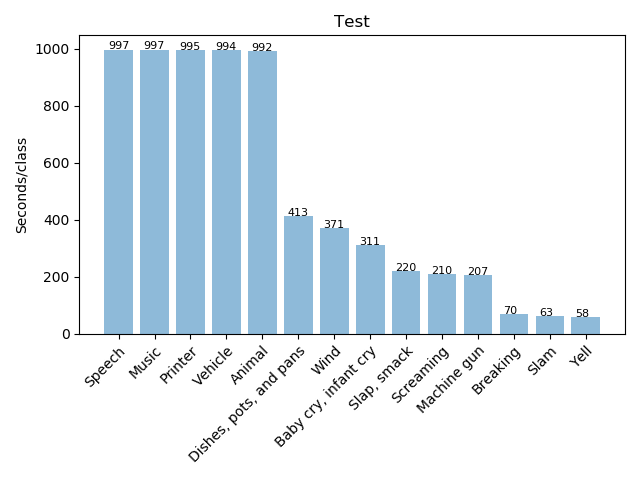
\includegraphics[width=0.5\linewidth]{tst_unbal_svm}
			\subcaption{This are the resulting subsets after downsampling the most populated classes and removing the zero-rows for the experiments that involve an SVM classifier}
		\end{subfigure}
		\vskip\baselineskip
		% Start with figure tfrecord
		\begin{subfigure}[b]{\textwidth}
			\centering
			\captionsetup{justification=centering}
			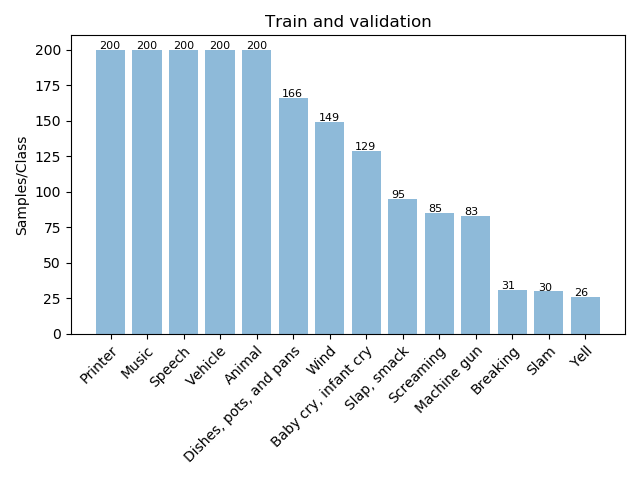
\includegraphics[width=0.5\linewidth]{tr_val_unbal}%
			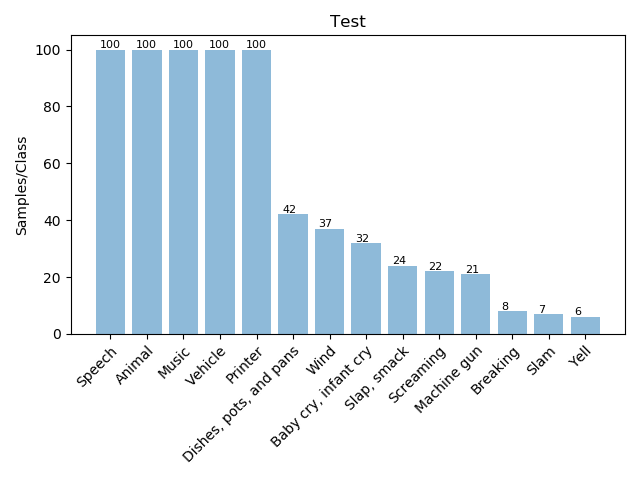
\includegraphics[width=0.5\linewidth]{tst_unbal}
			\subcaption{This are the resulting sets after downsampling the train and validation sets. The test set remains the same after the split.}
		\end{subfigure}
		
		\caption{Number of observations for train, validation and test subsets used in the different experiments}
		\label{fig:mesh15}
	\end{figure}
	
	
	\begin{table}[ht]
		\centering
		\begin{tabular}{|| m{5em} | m{9em} | m{9em} | m{9em} ||}
			\hline
			& \textbf{SVM multi and \acrshort{svm} + \acrshort{svm} binary} & \textbf{\acrshort{lstm} multi and \acrshort{lstm} + \acrshort{svm} binary} & \textbf{\acrshort{cnn} multi and \acrshort{cnn} + \acrshort{svm} binary}  \\
			\hline\hline
			\textbf{Train and validation} & 17645 (1993 per class) & 2800 (200 per class) & 2800 (200 per class) \\
			\hline
			\textbf{Test} & 6898 & 699 & 699 \\
			\hline                    
		\end{tabular}
		\caption{Train, validation and test set for different experiments}
		\label{table:8}
	\end{table}

\section{Implementations and results}

	For all the experiments, as mentioned above, the dataset was split by randomly selecting a 20\% of the data for the testing procedure. The other part was divided into train and validation subsets with a \acrlong{kfold} technique, with 10 folds, i.e. 10-fold cross-validation. A more detailed explanation about this resampling technique can be found in appendix \ref{appendix:kfold}. The average and standard deviation of the results from the different folds were obtained for train and validation. Then, a final measurement was performed for the test set. 
	
	The way of checking the model performance was by finding the accuracy and confusion matrix, whose explanation can be found in the Appendix \ref{appendix:metrics}. For the cross-validation procedure, a matrix with the average values\footnote{In the average matrices, the results for each cell are shown just with one decimal in order to make a better and more comfortable visualization. However, the colour bar on the right of the plots must be taking into account since there might be some cells in which the value shown is $0.0$ but it is actually greater.} was obtained and also one for the standard deviation\footnote{In the standard deviation matrices the results are shown multiplied by $10^{2}$ in order to see the value in the different cells of the matrix} so the estimation of the model is represented for the corresponding subsets. Finally, a last evaluation of the model is performed by checking the accuracy just once with the test set. The testing step is performed by using the model for which the highest value of accuracy for the validation fold was obtained during the train process.
	
	As mentioned above, we have develped a total of six final implementations. Three of them for a multiclass classification problem that consists of predicting the right label for each sample within the fourteen labels already explained. The other three are basically \acrshort{svm} binary classifiers that take as input the output probabilities of the multiclass classifications. The purpose of these three is to adapt the model to the final objective of creating a system to distinguish between violent and non-violent scenarios. In figure \ref{fig:mesh17}, two block diagrams are included in order to represent the flow in the multiclass and binary classification approaches.
	
	\begin{figure}[ht]
		% Whole figure
		\captionsetup{justification=centering}
		\begin{subfigure}[b]{\textwidth}
			% Start with figure wav
			\centering
			\captionsetup{justification=centering}
			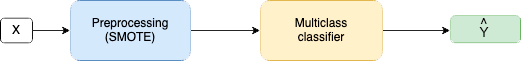
\includegraphics[scale=0.65]{multiclass-classifier}
			\caption{General model for the the three multiclass classification approaches.}
		\end{subfigure}
		\vskip\baselineskip
		% Start with figure tfrecord
		\begin{subfigure}[b]{\textwidth}
			\centering
			\captionsetup{justification=centering}
			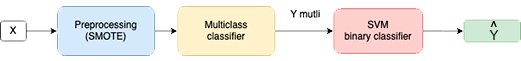
\includegraphics[scale=0.7]{mutli+svm-binary}
			\caption{Block diagram that shows the concatenation of multiclass classifier and the SVM binary classifier.}
		\end{subfigure}
		
		\caption{Confusion matrices for SVM multiclass classification for train and validation sets}
		\label{fig:mesh17}
	\end{figure}

	The output denoted as \textit{\^{Y} multi} corresponds to the predicted labels by the multiclass classifier. \todo{CPM: pero las etiquetas predichas son duras. En su día hablamos de tomar las blandas, ¿no?} Then, this feeds the binary classifier in order to be trained. The split for this process is also 20\% for the test set and the rest is split into train and validation with a \acrshort{kfold} algorithm. Then, the model instance for which the best accuracy value was obtained in the validation set is used for the testing process. \todo{CPM: pero ¿volviste a hacer la partición otra vez? ¿el testset del multi no es el del binario?}
	
\subsection{Implementation 1: \acrshort{svm} classifier for a multiclass classification}
\label{subsection:implementation-1}

	We decided to establish a baseline by making a first experiment based on a \acrshort{svm} classifier that is used for a multiclass classification. In this case, we wanted to check the results of the performance of one of the most employed techniques in this filed different from \acrshort{nn}. It is true that this method is originally designed for binary problems but, as explained in \ref{subsection:svm}, we took advantage fo the multiclass algorithm. To define our model, we used mainly the default parameters. In this work, we have not investigated which type of kernel could better fit our problem, however we found in the literature that the default option of \acrshort{rbf} is the most appropriated for real world applications \cite{Prajapati2010}. 
	
	Below, we can find the results for the different sets. In figure \ref{fig:mesh18}, the confusion matrices for the train and validation sets are shown. In figure \ref{fig:mesh19}, the confusion matrix for the evaluation on the test set is included. Finally, in the bar plot of figure \ref{fig:mesh20}, the accuracy values for the three sets are represented. For this case, the standard deviation is not shown for train and validation because it is zero when considering two decimals. \todo{CPM: ¿cómo has hecho esta desviación estándard? ¿Cada uno de los 10 modelos contra el test y el promedio y std? Es muy raro que salga 0}
	
	\begin{figure}[ht]
		% Whole figure
		\captionsetup{justification=centering}
		\begin{subfigure}[b]{\textwidth}
			% Start with figure wav
			\captionsetup{justification=centering}
			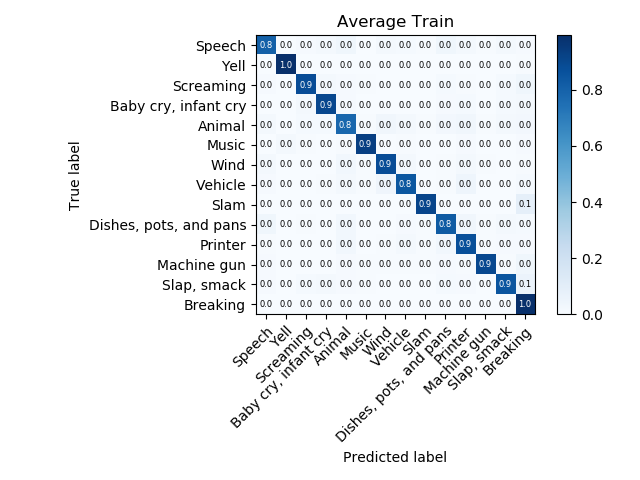
\includegraphics[width=0.6\linewidth]{svm-multi-cm-tr-av}%
			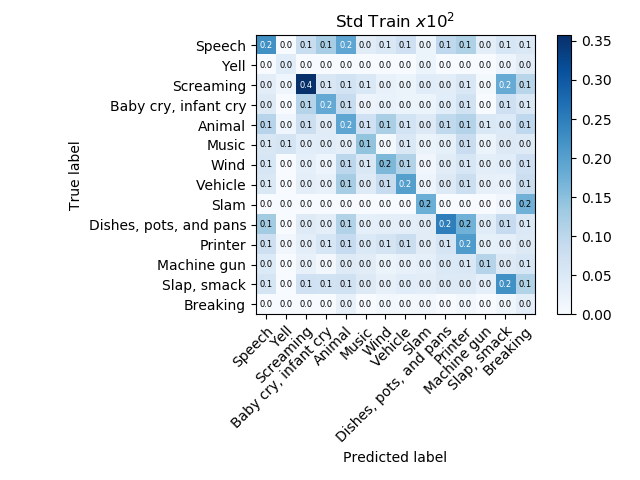
\includegraphics[width=0.6\linewidth]{svm-multi-cm-tr-std}
			\subcaption{Average and standard deviation for the train set}
		\end{subfigure}
		\vskip\baselineskip
		% Start with figure tfrecord
		\begin{subfigure}[b]{\textwidth}
			\captionsetup{justification=centering}
			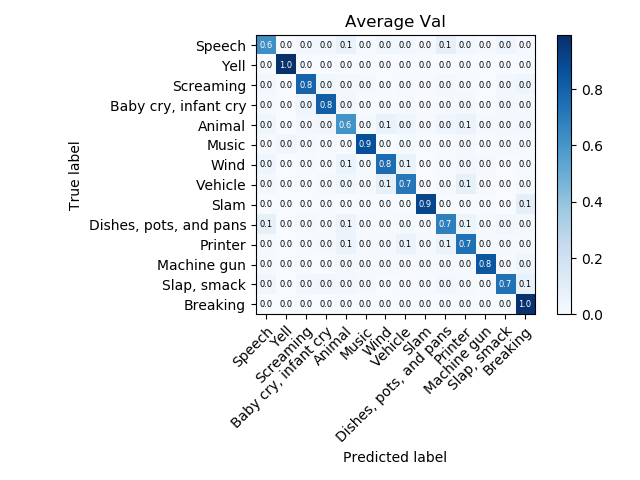
\includegraphics[width=0.6\linewidth]{svm-multi-cm-val-av}%
			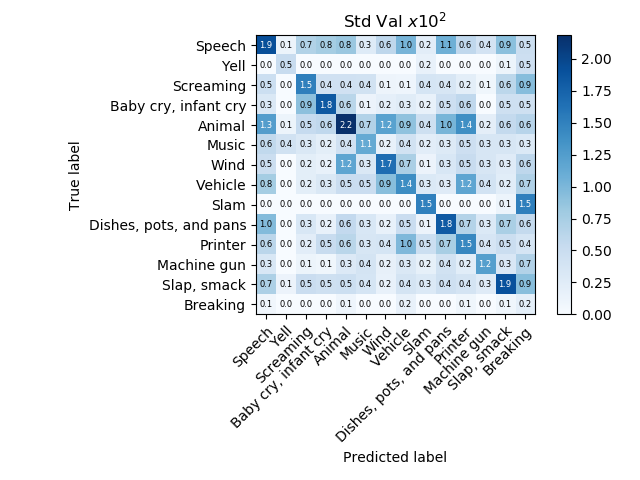
\includegraphics[width=0.6\linewidth]{svm-multi-cm-val-std}
			\subcaption{Average and standard deviation for the validation set}
		\end{subfigure}
		
		\caption{Confusion matrices for SVM multiclass classification for train and validation sets}
		\label{fig:mesh18}
	\end{figure}

	\begin{figure}[H]
		\centering
		\captionsetup{justification=centering}
		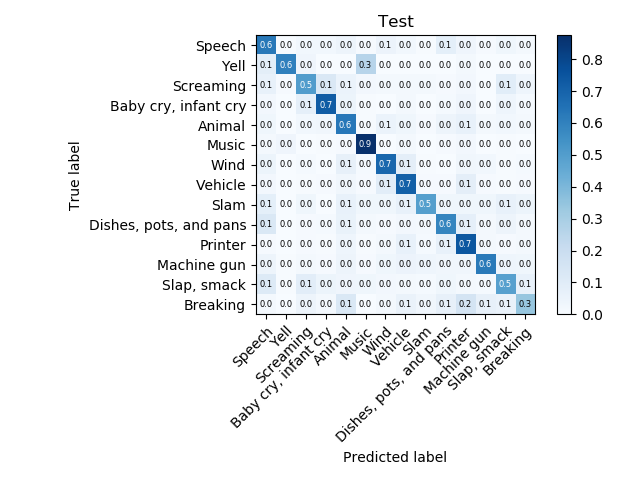
\includegraphics[width=0.7\linewidth]{svm-multi-cm-tst}
		\caption{Confusion matrix for the test set for the SVM multiclass classification}
		\label{fig:mesh19}
	\end{figure}

	\begin{figure}[H]
		\centering
		\captionsetup{justification=centering}
		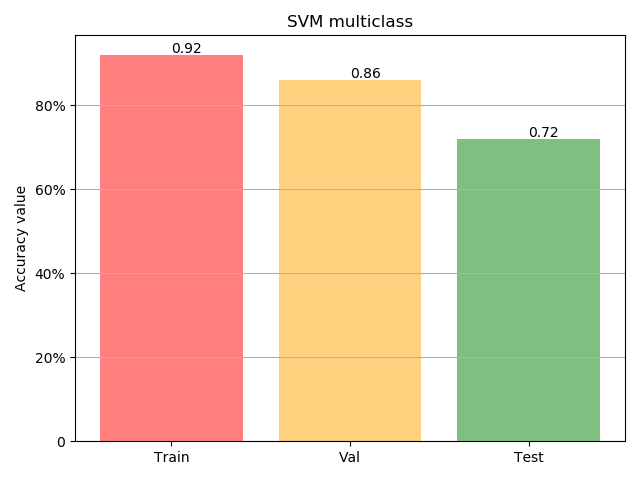
\includegraphics[width=0.7\linewidth]{svm-multierrorbar}
		\caption{Accuracy values for the three sets for the SVM multiclass classification}
		\label{fig:mesh20}
	\end{figure}
\todo{CPM: tienes que dar los valores de la desviación estándar de la accuracy}

	As we can see, the accuracy average values are a $92\%$ for the training set, a $86\%$ for the validation and $72\%$ for test. This can also be appreciated in the average confusion matrices. The diagonal for the training and the validation stands out the other cells but they do not present a sense of overfitting due to they are not completely uniform. In the test results, we can see greater values in the true positive sections for the most populated classes, mentioned above in section \ref{section:input-data-preparation}. This makes sense since the test set has more samples in these categories. We can consider a good result for this case. The accuracy of the final testing process is not much lower than the one obtained for the validation set. It would be a good option to populate more the violent labels, but we did not want to use synthetic data in the final evaluation.

\subsection{Implementation 2: \acrshort{svm} multiclass classification and \acrshort{svm} binary classification}

	The \acrshort{svm} multiclass model is then incorporated to the previous stage of the preprocessing. So, it predicts the multiclass probability for each value, what can also be interpreted as it is converting the data to a new feature space before the binary classification.
	
	The results in accuracy and confusion matrices for the different evaluations can be found below. Figure \ref{fig:mesh23} includes the average confusion matrices for train and validation sets. Then, figure \ref{fig:mesh24} shows the confusion matrix for the test set. Finally, in figure \ref{fig:mesh25}, the accuracy values for the three sets are shown, with their perspective standard deviations.
	
	\begin{figure}[H]
		\begin{center}
			% Whole figure
			\captionsetup{justification=centering}
			\begin{subfigure}[b]{\textwidth}
				% Start with figure wav
				\centering
				\captionsetup{justification=centering}
				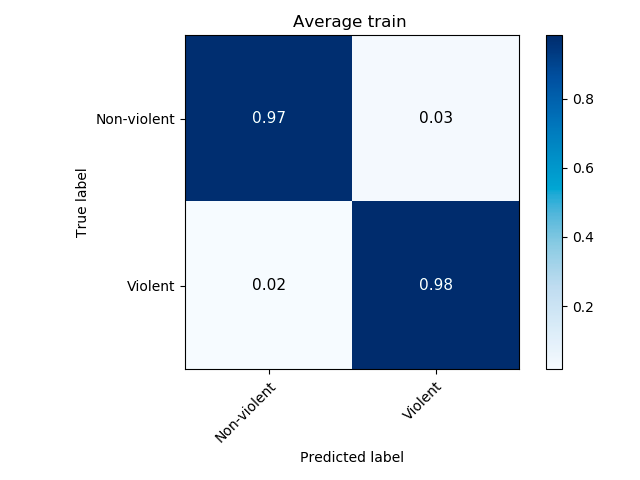
\includegraphics[width=0.55\linewidth]{svm-svm-cm-tr-av}%
				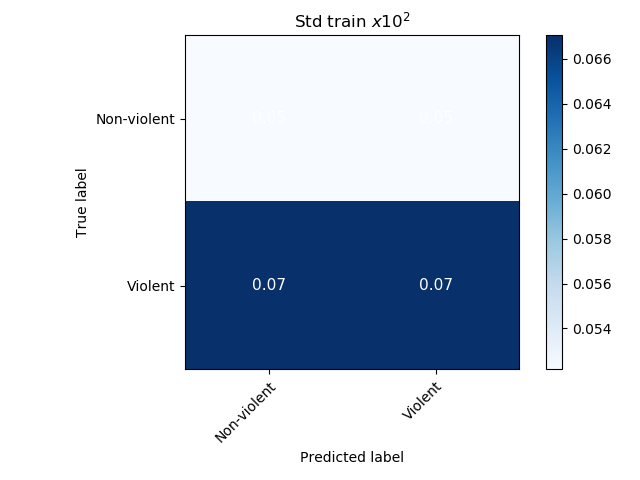
\includegraphics[width=0.55\linewidth]{svm-svm-cm-tr-std}
				\subcaption{Average and standard deviation for the train set}
			\end{subfigure}
			\vskip\baselineskip
			% Start with figure tfrecord
			\begin{subfigure}[b]{\textwidth}
				\centering
				\captionsetup{justification=centering}
				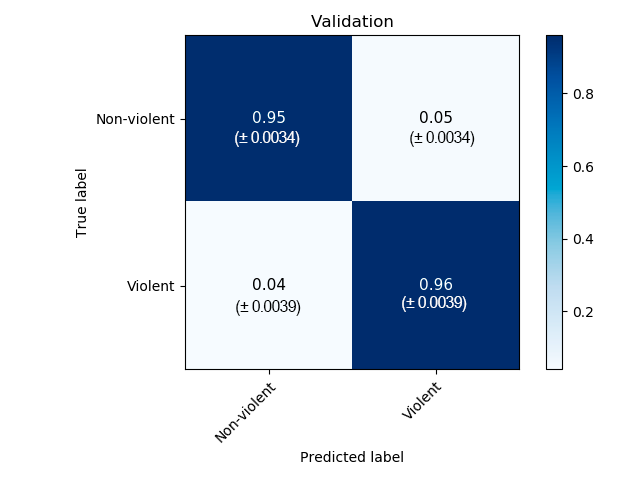
\includegraphics[width=0.55\linewidth]{svm-svm-cm-val-av}%
				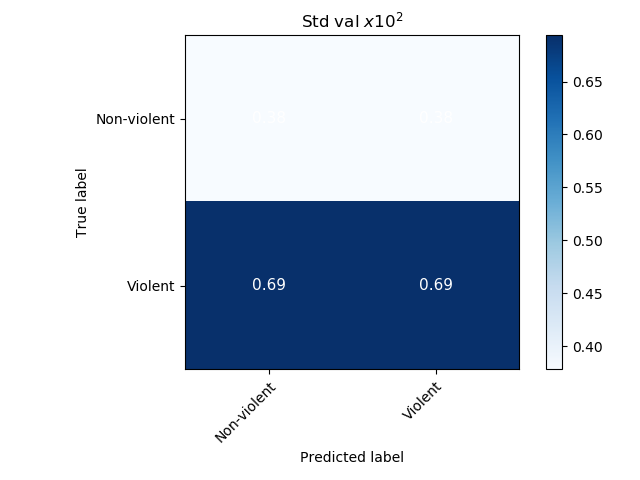
\includegraphics[width=0.55\linewidth]{svm-svm-cm-val-std}
				\subcaption{Average and standard deviation for the validation set}
			\end{subfigure}
			\caption{Confusion matrices for SVM multiclass + SVM binary classification}
			\label{fig:mesh23}
		\end{center}
	\end{figure}
	
	\begin{figure}[H]
		\centering
		\captionsetup{justification=centering}
		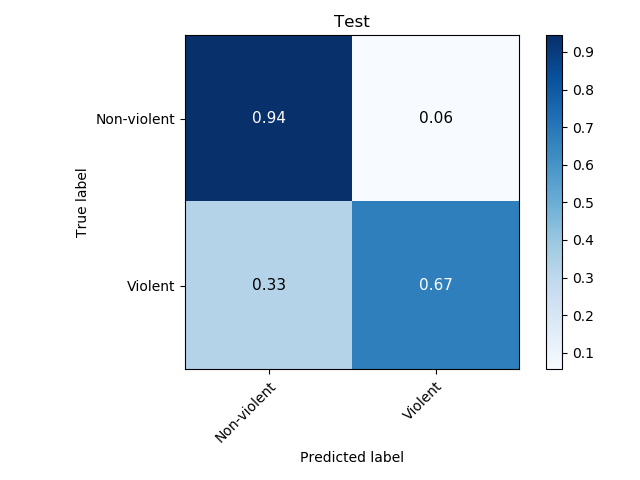
\includegraphics[width=0.7\linewidth]{svm-svm-cm-tst}
		\caption{Confusion matrix for the test set for the SVM multiclass + SVM binary classification}
		\label{fig:mesh24}
	\end{figure}

	In this performing model it is more important to pay attention to both metrics. In the accuracy bar plot, at first, it can be interpreted that the results are really good. This can be due to the high number of samples for a binary classification. Considering the test value of 91\%, we can see that the merit of the good performance is thank to the good classification of the non-violent observations, while the result on differentiating the violent classes is not as good since just the 60\% of the labels were correctly predicted. For the train and validation sets, the results are pretty good for both types, being a 98\% for both cases. Again, the fact of creating a big amount of the samples artificially for the training and validating parts is given a considerable difference in the results respect to the testing. However, this output also allows that with a more balanced test set the performance would be more even in the tree sets, as it happened with the multiclass task explained before, and that those observations which belong to the original embeddings show a satisfying outcome.
	
	\todo{CPM: tienes que mostrar también el resultado binario de hacer la clasificación simplemente teniendo en cuenta los resultados multiclases sabiendo cuáles clases son violentas y cuales no. Esto que hablamos de utilizar las salidas duras o las blandas. El resultado debería ser peor... }
	
	\begin{figure}[H]
		\centering
		\captionsetup{justification=centering}
		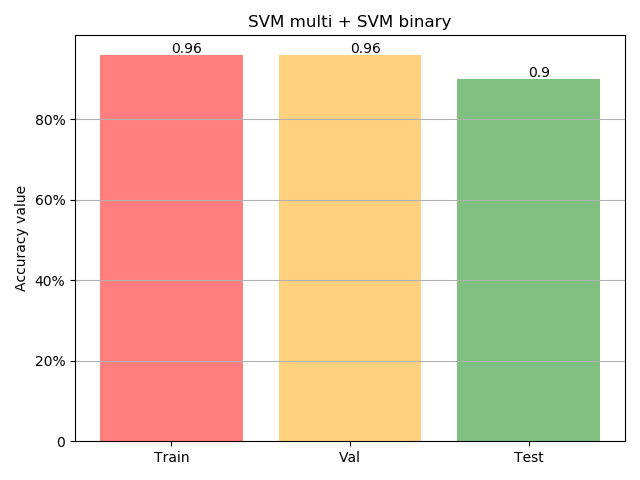
\includegraphics[width=0.7\linewidth]{svm-binaryerrorbar}
		\caption{Accuracy values for the three sets for the SVM multiclass + SVM binary classification}
		\label{fig:mesh25}
	\end{figure}
	\todo{CPM: tienes que dar los valores de la desviación estándar de la accuracy}
	
\subsection{Implementation 3: \acrshort{lstm} for multiclass classification}

	\begin{wrapfigure}{r}{0.35\textwidth}
		\centering
		\captionsetup{justification=centering}
		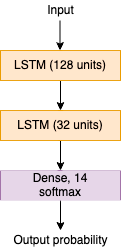
\includegraphics[width=0.5\linewidth]{lstm}
		\caption{LSTM architecture}
		\label{fig:mesh26}
	\end{wrapfigure}
	
	For this implementation we have decided to use a network composed by a total of three layers: two \acrshort{lstm} and a final \acrlong{fc} with a softmax activation function for the classification task. The first two \acrshort{lstm} layers are set with a drop-out of 0.05 and a recurrent dropout of 0.35. For the first one, the number of units was set to 128, in order not to change the dimensions of its output. In the second layer, it was set to 32 layers so as to reduce the dimensionality before the final prediction in the dense layer. In figure \ref{fig:mesh26}, an schema of the model is shown.
	
	The function minimized in the process was the categorical cross-entropy, which is a common way to evaluate multiclass classification problems. A more detailed explanation of this function can be found in appendix \ref{appendix:categorical-cross-entropy}. With respect to the training process, a number of 50 epochs were used and also a batch size of 32 samples \footnote{When training a machine learning model, an optimization algorithm, usually \acrshort{sgd}, is in charge of updating the internal parameters so a good performance is achieved and the loss function can be minimized. The epochs is a hyperparameter that establishes how many times the learning algorithm pass through the entire train set in the training process. The batch size is the one that defines the number of observations the algorithm works through before assigns the internal parameters an updated value \cite{Browniee2018a}}. \todo{remove from footnote. CPM: no entiendo qué quieres quitar pero es demasiado genérico si dices que se suele usar SGD. Di si lo usas o no.} Also, a \acrshort{nadam} optimizer was used and a learning rate of $2e^{-3}$.
	
	Below, the results for the classification are included. In figure \ref{fig:mesh27}, the average and standard deviation matrices for the train and validation sets are shown. Then, in figure \ref{fig:mesh28}, the confusion matrix for the testing process is included. In figure \ref{fig:mesh29}, a bar plot shows the accuracy for every set with their standard deviation values.
	
		\begin{figure}[H]
		% Whole figure
		\captionsetup{justification=centering}
		\begin{subfigure}[b]{\textwidth}
			\centering
			% Start with figure wav
			\captionsetup{justification=centering}
			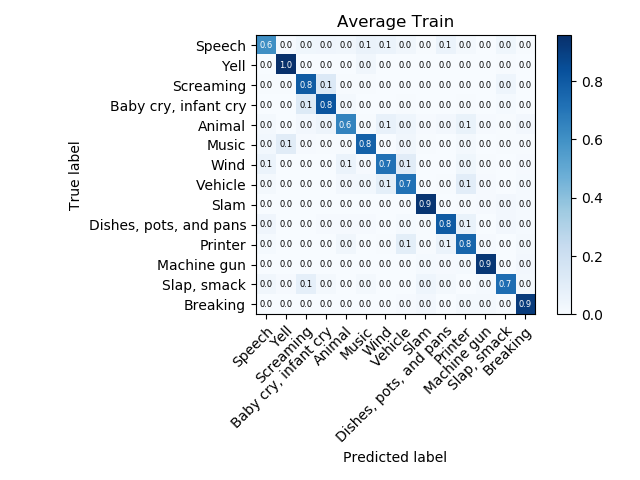
\includegraphics[width=0.6\linewidth]{lstm-multi-cm-tr-av}%
			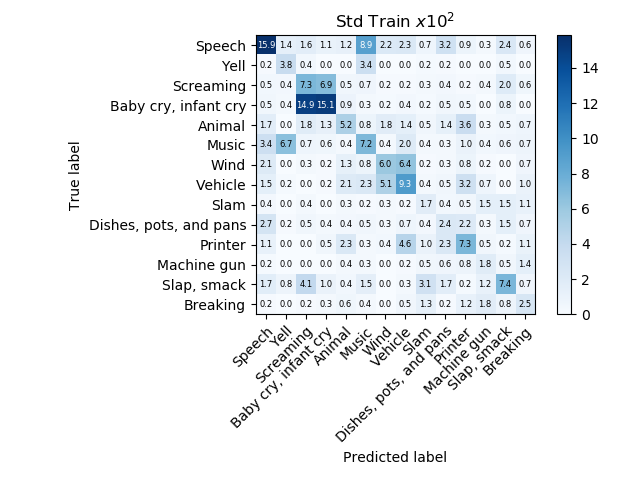
\includegraphics[width=0.6\linewidth]{lstm-multi-cm-tr-std}
			\subcaption{Average and standard deviation for the train set}
		\end{subfigure}
		\vskip\baselineskip
		% Start with figure tfrecord
		\begin{subfigure}[b]{\textwidth}
			\centering
			\captionsetup{justification=centering}
			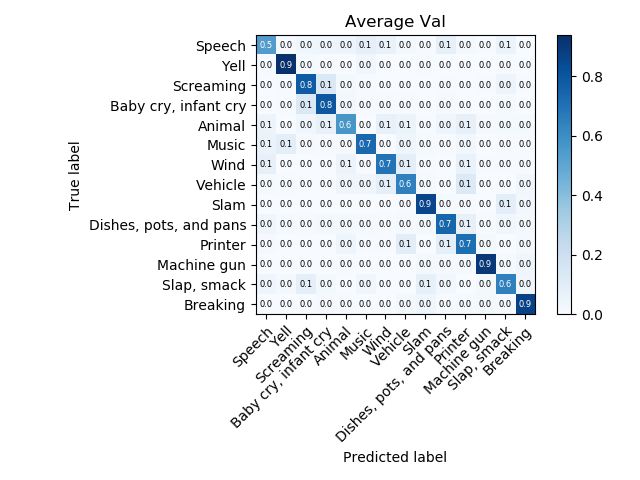
\includegraphics[width=0.6\linewidth]{lstm-multi-cm-val-av}%
			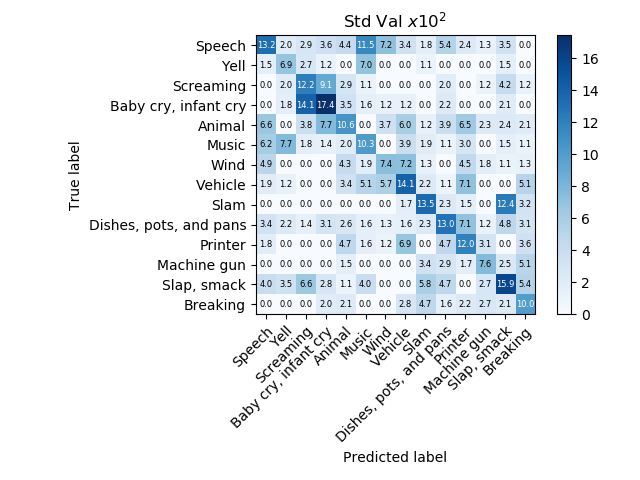
\includegraphics[width=0.6\linewidth]{lstm-multi-cm-val-std}
			\subcaption{Average and standard deviation for the validation set}
		\end{subfigure}
		\caption{Confusion matrices for LSTM multiclass classification for train and validation sets}
		\label{fig:mesh27}
	\end{figure}
	
	\begin{figure}[H]
		\centering
		\captionsetup{justification=centering}
		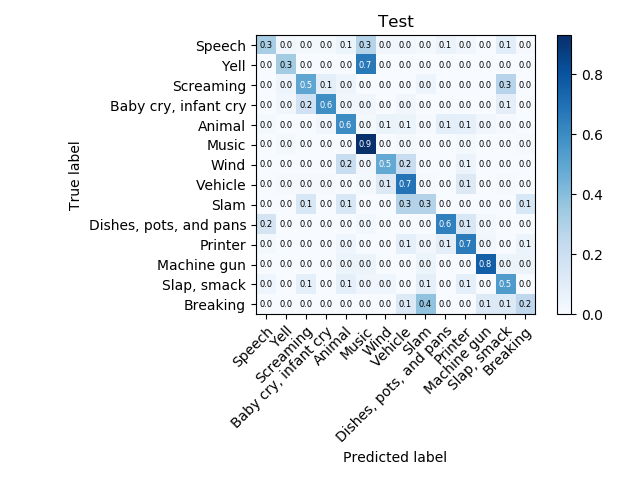
\includegraphics[width=0.7\linewidth]{lstm-multi-cm-tst}
		\caption{Confusion matrix for the test set for the LSTM multiclass classification}
		\label{fig:mesh28}
	\end{figure}
	
	\begin{figure}[H]
		\centering
		\captionsetup{justification=centering}
		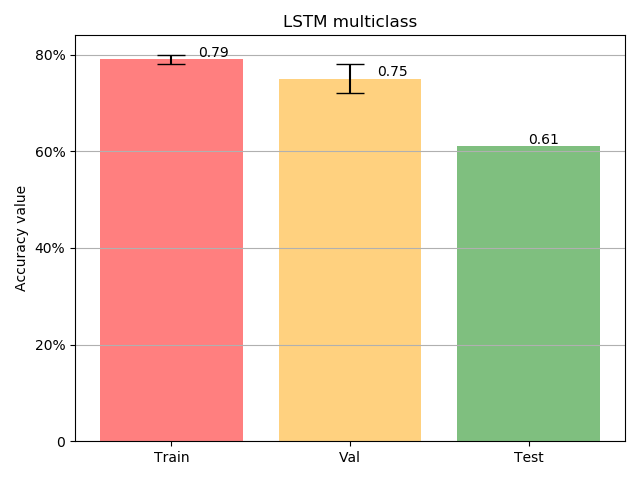
\includegraphics[width=0.7\linewidth]{lstm-multierrorbar}
		\caption{Accuracy values for the three sets for the LSTM multiclass classification}
		\label{fig:mesh29}
	\end{figure}

	\todo{CPM: ahora está bien que aparezcan las desviaciones pero la del test, ¿no sale porque se ha hecho con el mejor modelo? Esto es lo que te preguntaba con la SVM que te sale la std práctimente 0}

	For this model, we obtained an accuracy of $79\% \pm 1\%$ for the training set, a $75\% \pm 3\%$ for the validation and a $61\%$ for the test. This can be due to the possible confusion regions mainly between classes such as \textit{Screaming} and \textit{Baby cry, infant cry}, and \textit{Wind} and \textit{Vehicle}, whose standard deviation values are the most emphasized. In the testing procedure, a really good performance was done for the class \textit{Yell}. The other violent classes have fewer correct predictions but also due to the fewer samples that belong to these classes in the test subset. We can discard heavy overfitting since the values of accuracy in the training and validation sets with respect to the test one are not too different. %away from each other.
	
\subsection{Implementation 4: \acrshort{lstm} multiclass + \acrshort{svm} for a final binary classification}
	
	For this case, the predicted probabilities obtained from the \acrshort{lstm} multiclass classifier are passed as input to the \acrshort{svm} for the binary classification. 
	
	The accuracy value for the different sets are included. Figure \ref{fig:mesh30} shows the average confusion matrices for the train and validation sets. In figure \ref{fig:mesh31}, the confusion matrix for the test set is also included, and in figure \ref{fig:mesh32}, the error bar can be seen with the accuracy values for each of the sets.
	
	\begin{figure}[H]
		\begin{center}
			% Whole figure
			\captionsetup{justification=centering}
			\begin{subfigure}[b]{\textwidth}
				% Start with figure wav
				\centering
				\captionsetup{justification=centering}
				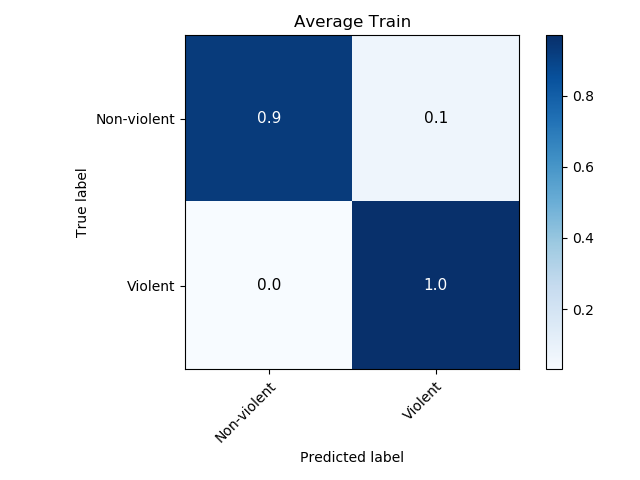
\includegraphics[width=0.55\linewidth]{lstm-svm-cm-tr-av}%
				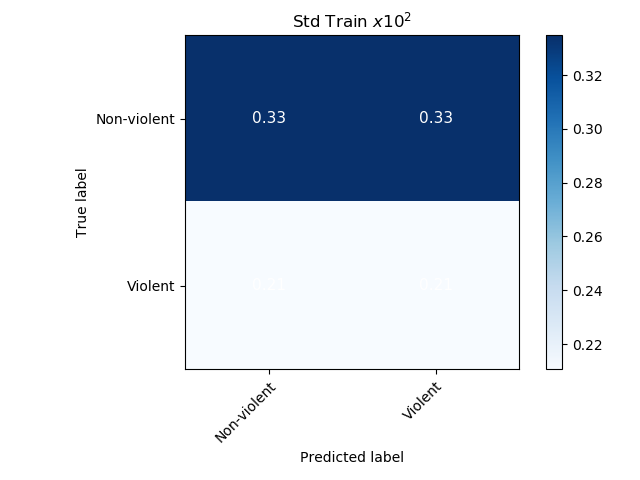
\includegraphics[width=0.55\linewidth]{lstm-svm-cm-tr-std}
				\subcaption{Average and standard deviation for the train set}
			\end{subfigure}
			\vskip\baselineskip
			% Start with figure tfrecord
			\begin{subfigure}[b]{\textwidth}
				\centering
				\captionsetup{justification=centering}
				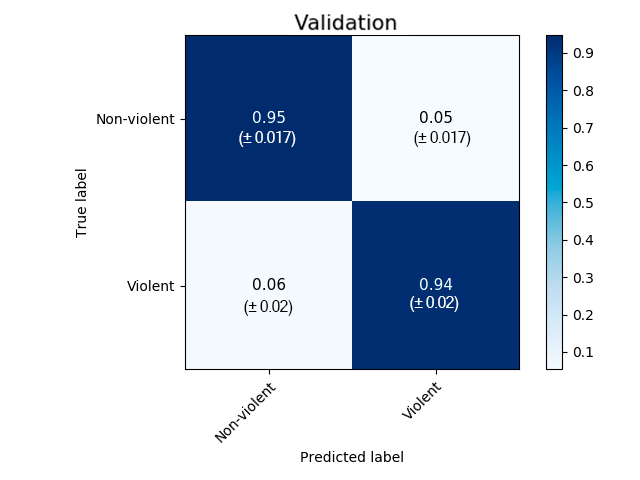
\includegraphics[width=0.55\linewidth]{lstm-svm-cm-val-av}%
				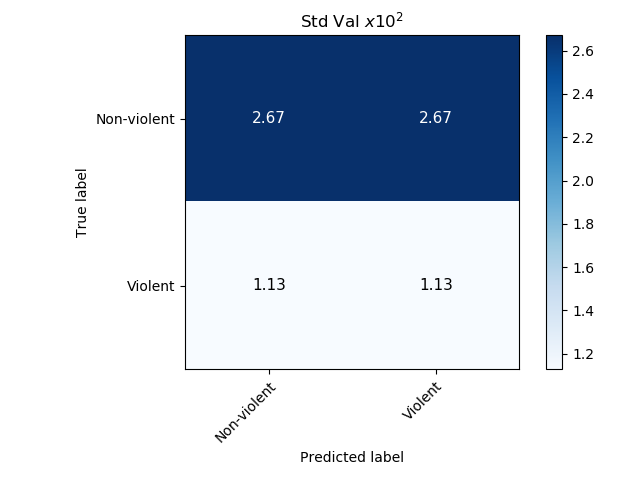
\includegraphics[width=0.55\linewidth]{lstm-svm-cm-val-std}
				\subcaption{Average and standard deviation for the validation set}
			\end{subfigure}
			\caption{Confusion matrices for LSTM multiclass + SVM binary classification}
			\label{fig:mesh30}
		\end{center}
	\end{figure}
	
	\begin{figure}[H]
		\centering
		\captionsetup{justification=centering}
		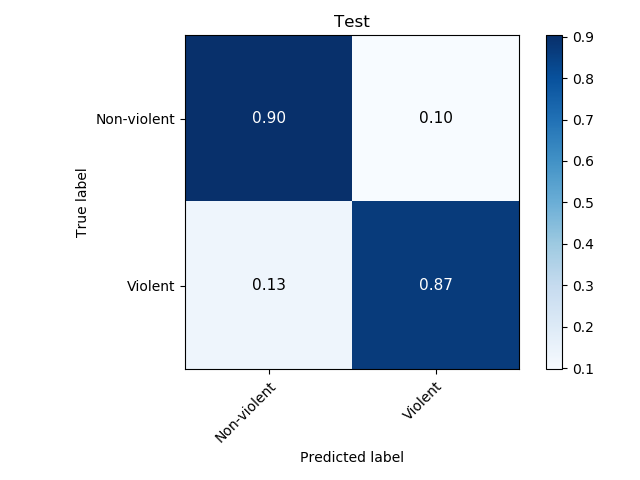
\includegraphics[width=0.7\linewidth]{lstm-svm-cm-tst}
		\caption{Confusion matrix for the test set for the LSTM multiclass + SVM binary classification}
		\label{fig:mesh31}
	\end{figure}
	
	\begin{figure}[H]
		\centering
		\captionsetup{justification=centering}
		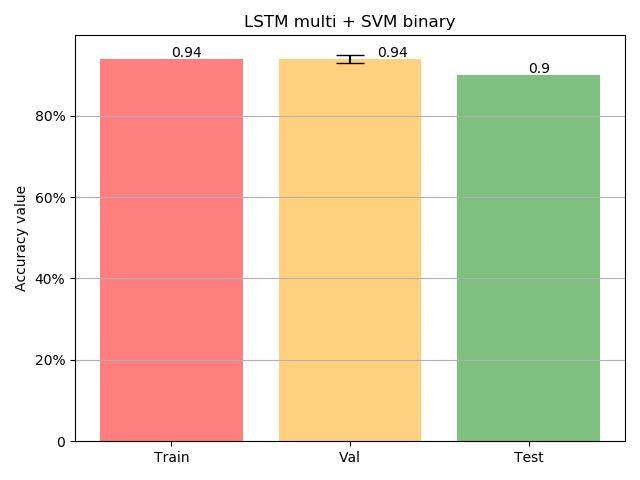
\includegraphics[width=0.7\linewidth]{lstm-svmerrorbar}
		\caption{Accuracy values for the three sets for the LSTM multiclass + SVM binary classification}
		\label{fig:mesh32}
	\end{figure}

	As shown in the bar plot, the values of the accuracy for train and validation are $95\%$ and $95\% \pm 1\%$, respectively. The average matrices are really good as well. The no variation between them could be understood as a symptom of overfitting. However, the accuracy for testing is $90\%$, which is similar to the train and test results. The interesting point can be read in the confusion matrix for the test set. The classification of the violent classes is almost as good as the one for the non-violent ones, despite of the less amount of samples in these categories. 

	
\subsection{Implementation 5: \acrshort{cnn} for multiclass classification}

	For this case, we have implemented a \acrshort{cnn} model based on the architecture presented in figure \ref{fig:mesh5} in subsection \ref{subsection:exploring-differences-between-two-types-of-data-access} for the small experiment to check the similarity of the embeddings from the .\textit{tfrecord} files and the naturally audio files.
	
	In the configuration of the network, the same hyperparameters from implementation 3 are used for the learning process: a categorical cross-entropy for the loss function, a \acrshort{nadam} optimizer, a number of 50 epochs and a batch size of 32 samples. We have kept the same value for this model since the number of observations is the same and the depth of the network is not very great. A learning rate of $2e^{-3}$ was also used. 
	
	In figure \ref{fig:mesh33}, the average and standard deviation matrices for the train and validation sets are shown. In figure \ref{fig:mesh34}, the confusion matrix for the test set. The bar plot in \ref{fig:mesh35}, shows the accuracy for every set with their standard deviation values.
	
	\begin{figure}[H]
		\begin{center}
		% Whole figure
		\captionsetup{justification=centering}
		\begin{subfigure}[b]{\textwidth}
			% Start with figure wav
			\centering
			\captionsetup{justification=centering}
			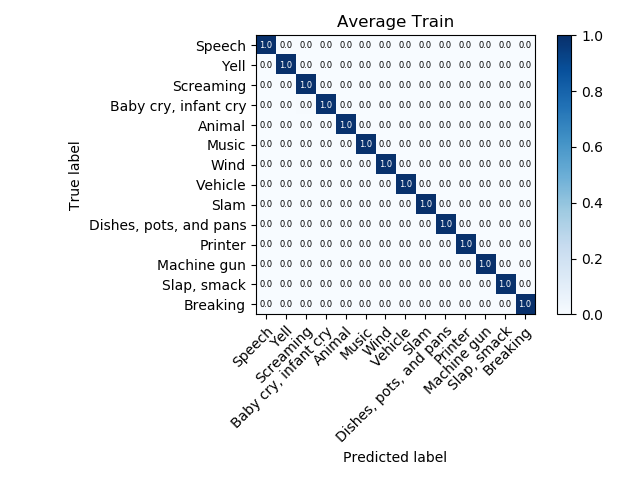
\includegraphics[width=0.55\linewidth]{cnn-multi-cm-tr-av}%
			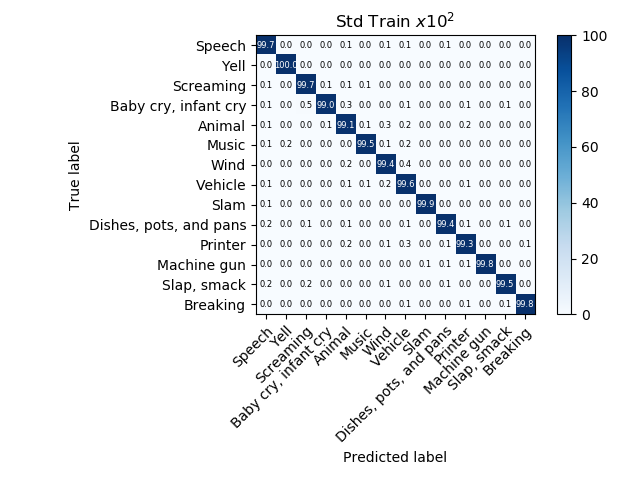
\includegraphics[width=0.55\linewidth]{cnn-multi-cm-tr-std}
			\subcaption{Average and standard deviation for the train set}
		\end{subfigure}
		\vskip\baselineskip
		% Start with figure tfrecord
		\begin{subfigure}[b]{\textwidth}
			\centering
			\captionsetup{justification=centering}
			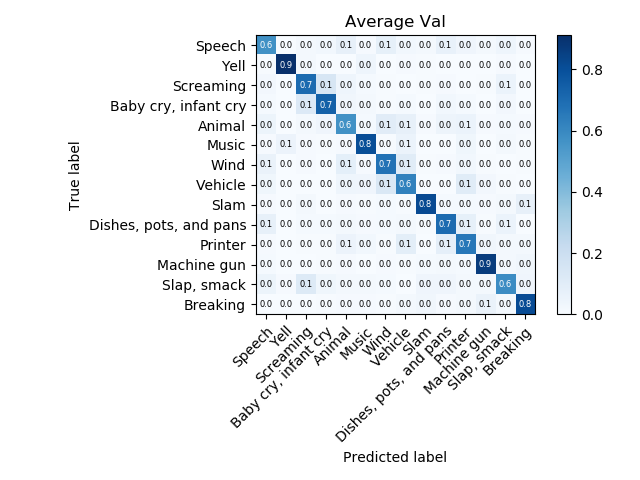
\includegraphics[width=0.55\linewidth]{cnn-multi-cm-val-av}%
			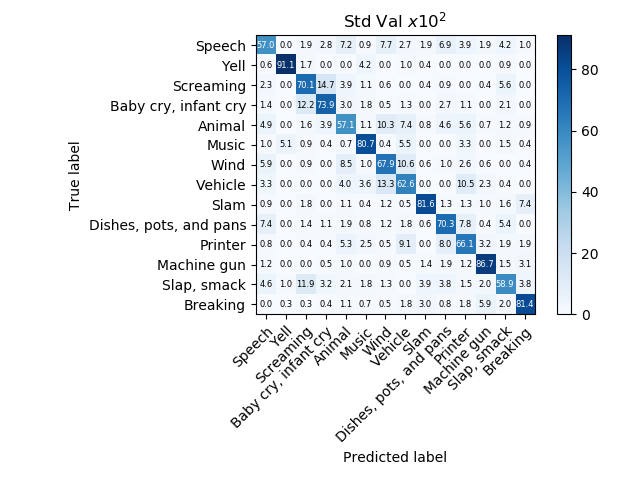
\includegraphics[width=0.55\linewidth]{cnn-multi-cm-val-std}
			\subcaption{Average and standard deviation for the validation set}
		\end{subfigure}
		\caption{Confusion matrices for CNN multiclass classification for train and validation sets}
		\label{fig:mesh33}
		\end{center}
	\end{figure}
	
	\begin{figure}[H]
		\centering
		\captionsetup{justification=centering}
		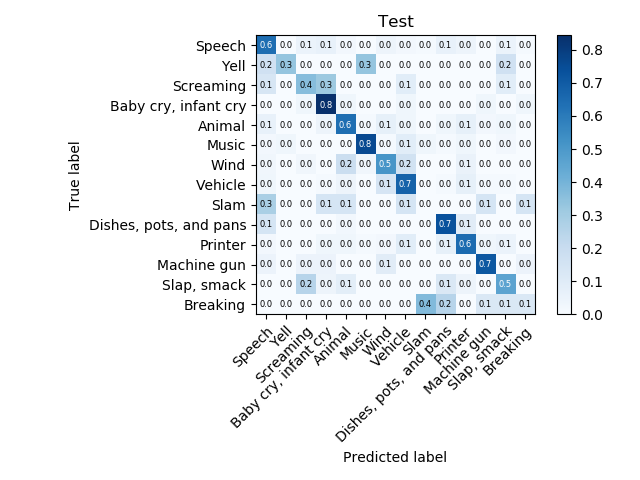
\includegraphics[width=0.7\linewidth]{cnn-multi-cm-tst}
		\caption{Confusion matrix for the test set for the CNN multiclass classification}
		\label{fig:mesh34}
	\end{figure}
	
	\begin{figure}[H]
		\centering
		\captionsetup{justification=centering}
		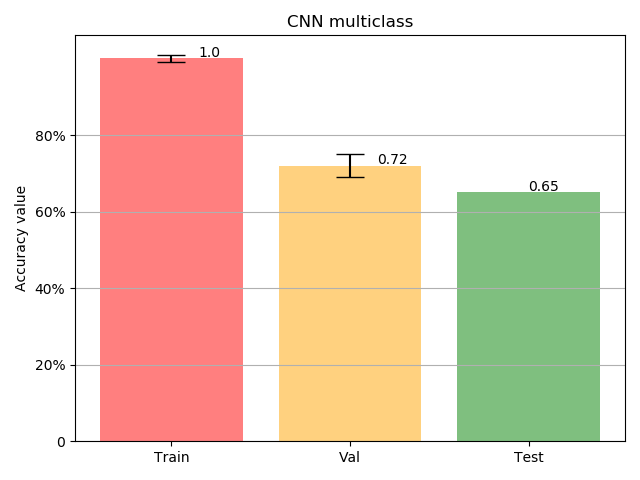
\includegraphics[width=0.7\linewidth]{cnn-multierrorbar}
		\caption{Accuracy values for the three sets for the CNN multiclass classification}
		\label{fig:mesh35}
	\end{figure}

	The values of the accuracy obtained for this implementation are $98\% \pm 1\%$ for the train set, $72\% \pm 3\%$ for validation and $65\%$ for the test set. In the error bar in figure \ref{fig:mesh35}, the difference between the red bar for train is considerable meaningful with respect to the other two. Also, the confusion matrix for train shows a very well marked diagonal, while the other two are not that perfect. In the validation set, there are some misclassifications but still the equality among cells is present. Some confusion regions can be found again between \textit{Screaming} and \textit{Baby cry, infant cry} or \textit{Wind} and \textit{Vehicle}. In the test set, we can see that the diagonal does not follow a regular shape, being this one the worst result of the experiments.

\subsection{Implementation 6: \acrshort{cnn} multiclass + \acrshort{svm} for a final binary classification}

	In this last approach we wanted to use the predictions from the \acrshort{cnn} to feed the binary classifier \acrshort{svm}.
	
	Figure \ref{fig:mesh36} shows the average of the confusion matrices for the train and validation sets. In figure \ref{fig:mesh37}, it is included the confusion matrix for the test set. Finally, figure \ref{fig:mesh38} shows the error bar in which the accuracy values for the three test can be seen.
	
	\begin{figure}[H]
		\begin{center}
			% Whole figure
			\captionsetup{justification=centering}
			\begin{subfigure}[b]{\textwidth}
				% Start with figure wav
				\centering
				\captionsetup{justification=centering}
				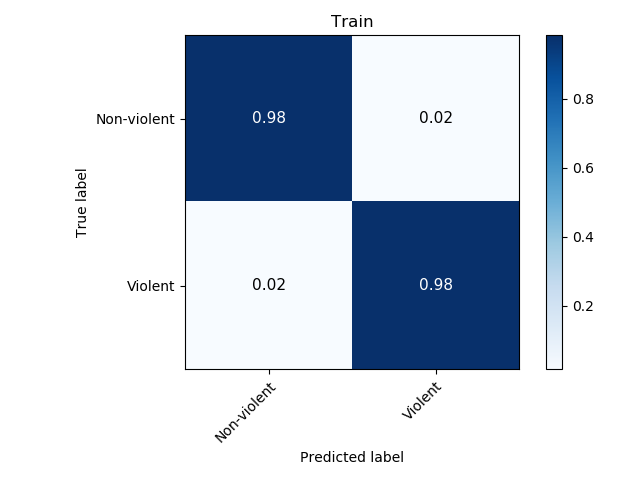
\includegraphics[width=0.55\linewidth]{cnn-svm-cm-tr-av}%
				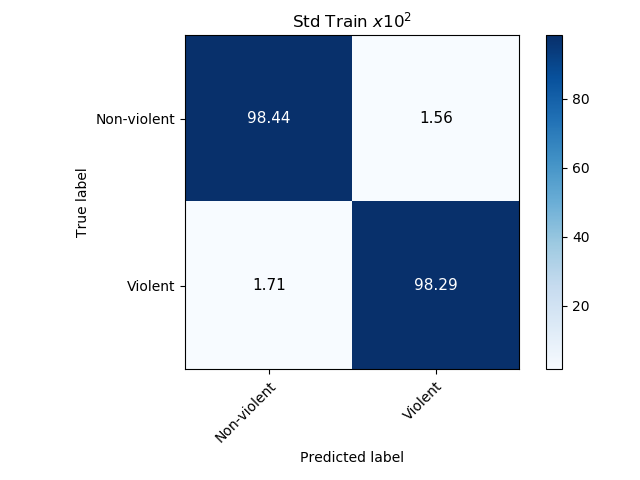
\includegraphics[width=0.55\linewidth]{cnn-svm-cm-tr-std}
				\subcaption{Average and standard deviation for the train set}
			\end{subfigure}
			\vskip\baselineskip
			% Start with figure tfrecord
			\begin{subfigure}[b]{\textwidth}
				\centering
				\captionsetup{justification=centering}
				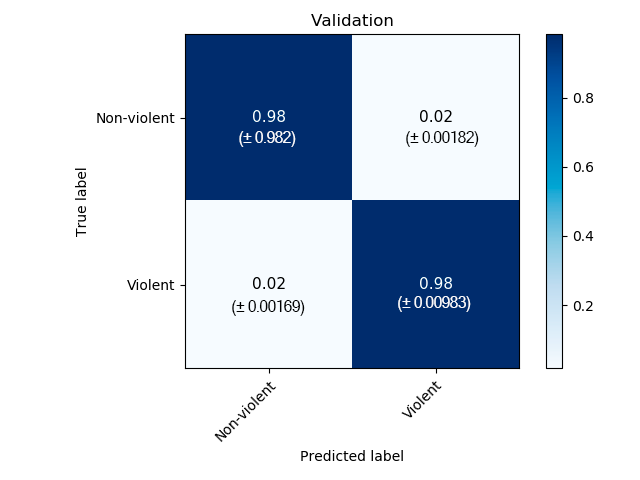
\includegraphics[width=0.55\linewidth]{cnn-svm-cm-val-av}%
				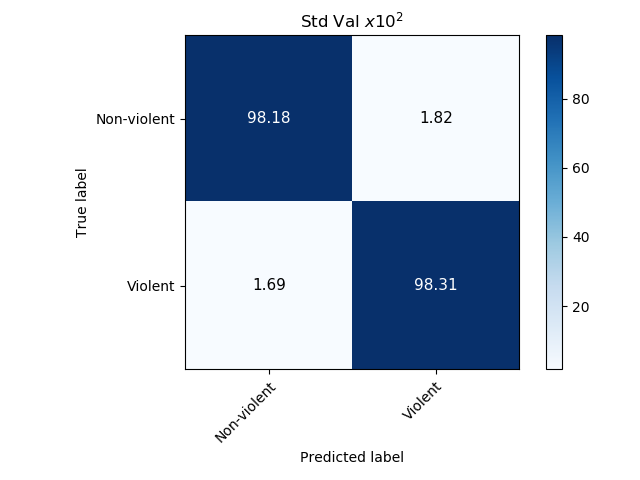
\includegraphics[width=0.55\linewidth]{cnn-svm-cm-val-std}
				\subcaption{Average and standard deviation for the validation set}
			\end{subfigure}
			\caption{Confusion matrices for CNN multiclass + SVM binary classification}
			\label{fig:mesh36}
		\end{center}
	\end{figure}
	
	\begin{figure}[H]
		\centering
		\captionsetup{justification=centering}
		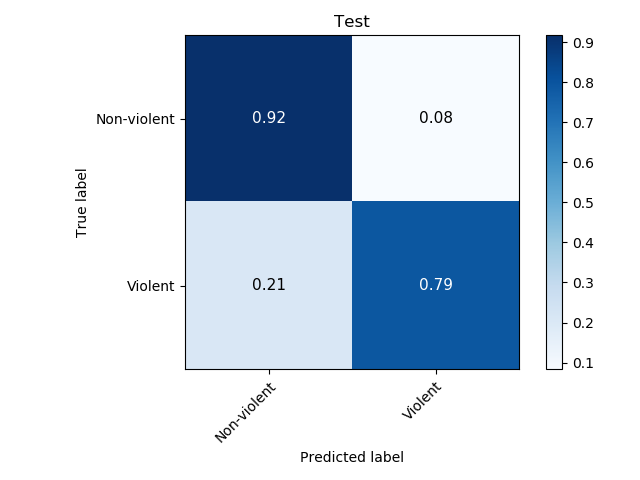
\includegraphics[width=0.7\linewidth]{cnn-svm-cm-tst}
		\caption{Confusion matrix for the test set for the CNN multiclass + SVM binary classification}
		\label{fig:mesh37}
	\end{figure}
	
	\begin{figure}[H]
		\centering
		\captionsetup{justification=centering}
		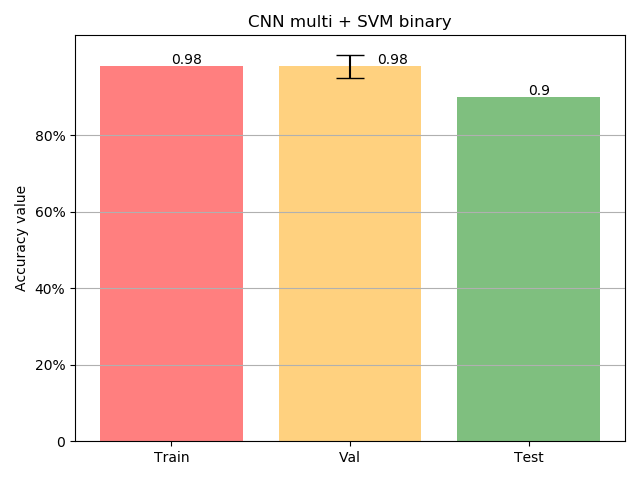
\includegraphics[width=0.7\linewidth]{cnn-svmerrorbar}
		\caption{Accuracy values for the three sets for the CNN multiclass + SVM binary classification}
		\label{fig:mesh38}
	\end{figure}

	The values of the accuracy are $98\%$, $98\% \pm 3\%$ and $90\%$ for train, validation and test set, respectively. Again the results are similar to the ones obtained in the experiment 4. In this case, the classification of the violent classes are good enough as well for the test. However, as seen in experiment 5, there are plenty of misclassifications for the test set but some of them happen between classes of the same kind, so this failures do not have an effect on the binary problem. Also, others have been \doubt{mixed} with categories from the other group, this is would be the reason of the lower output. 
	
\section{Comparison and conclusion}
	
	The idea behind the different implementations was to check the usefulness of the embeddings extracted with \acrshort{vgg}ish for a violent/non-violent classification problem. We wanted to study the performance of different learning techniques to see how this type of data worked with them. To do so, we first ran a typical algorithm for classification that does not involve \acrlong{nn}, an \acrshort{svm}. Then, we thought it could be a good idea to try neural models with different core concepts to exploit the nature of our data. The dimensions of our data allowed the use of the \acrshort{cnn}, while the sequential character of an audio instance makes the \acrshort{lstm} a possible approach. In this section, we are going to compare the six different results dividing the explanations according to the type classification: multiclass or binary. For the multiclass problem, the results are shown again in table \ref{table:9}
	
	\begin{table}[h!]
		\begin{center}
			\resizebox{0.7\columnwidth}{!}{%
			\begin{tabular}{|| m{5em} | m{7em} | m{7em} | m{7em} ||}
				\hline
				& \textbf{Train} & \textbf{Validation} & \textbf{Test} \\
				\hline\hline
				\textbf{SVM} & $92\%$ & $86\%$ & $72\%$ \\
				\hline
				\textbf{\acrshort{lstm}} & $79\% \pm 1\%$ & $75\% \pm 3\%$ & $61\%$ \\
				\hline
				\textbf{\acrshort{cnn}} & $98\% \pm 2\%$ & $72\% \pm 3\%$ & $65\%$ \\
				\hline
			\end{tabular}
		}
		\end{center}
		\caption{Accuracy results for the three different algorithms and the three sets}
		\label{table:9}
	\end{table}

	Initially, the best performance for this case is the one done by with \acrshort{svm}. It is expectable that this algorithm achieves a good result due to the way it works. Basically, it expresses the different data samples in a feature space in which the optimal boundary is computed, as explained in subsection \ref{subsection:svm}. However, this one is not totally comparable with the other two \acrshort{lstm} and \acrshort{cnn}, since the number of observations to feed the model is much greater because of the conversions explained in the subsection \ref{section:input-data-preparation}. This way, the method has more examples to learn how the different classes are distributed.
	
	For the \acrshort{cnn} approach, the results are maybe the least satisfactory. The system presents a clear overfitting due to the big difference of the results for within the three sets. It is learning the data in the training stage and not performing a not being able to generalize so as to perform a good enough classification for validation and test. Also, considering the errors in figure \ref{fig:mesh34}, the mismatches are the greatest of the three experiments.
	
	In the \acrshort{lstm} approach, the results are numerically the worst but also the ones that make more sense. The system does not present an overfitting since the accuracies for validation and test are similar to the one for train. Also, the errors that can be read in the confusion matrix in figure \ref{fig:mesh31} are understandable since the audio data for those classes involved in the confusion regions may look similar. For example, a recording that belongs to \textit{Baby cry, infant cry} is likely to be similar to one from \textit{Screaming}. The same explanation could be used for \textit{Wind} and \textit{Vehicle}, since they usually have sounds that belong to scenes in a rush.
	
	Let's look at some violent categories to check their performance. 
	
	\begin{itemize}
		\item The error when predicting \textit{Music} for \textit{Yell} samples that appears in \acrshort{svm} and \acrshort{cnn} results, is not a problem in the classification of the test set for the \acrshort{lstm}. In fact, all the \textit{Yell} samples belong to the true positive cell.
		\item The confusion region between \textit{Screaming} and \textit{Baby cry, infant cry} comes out in all matrices. This makes sense, since the semantics of these two type of audio events is quite similar.
		\item The predictions for \textit{Slam} are more or less the same between the \acrshort{svm} and \acrshort{lstm}, obtaining a true positive rate of $40\%$ and a distribution of the false negatives along all the other categories. For the \acrshort{cnn}, this class is a complete failure being most of it classified as \textit{Speech}.
		\item In the case of \textit{Machine gun} it has a pretty good performance for all the three models, getting a $70\%$ for \acrshort{lstm} and \acrshort{cnn} and a $60\%$ for the \acrshort{svm} of the samples as true positives. The rest of them are shared uniformly along all the other classes.
		\item In the case of \textit{Slap, smack}, it is predicted in a similar way for all the models as well, achieving a $50\%$ of the samples right classified.
		\item The class \textit{Breaking} has achieved similar results in \acrshort{svm} and \acrshort{lstm} being this last a $10\%$ absolute better. In the case of the \acrshort{cnn} model, it was mainly predicted as \textit{Slam}, being the true positive cell with just a $10\%$.
	\end{itemize}
	
   The conclusion we can extract from this comparison is that the model that shows a much better result in the sense of violent categories is the \acrshort{lstm}. However, when looking at the non-violent ones, the \acrshort{svm} makes a better performance, achieving the highest value for \textit{Music} with a $90\%$. The best system to keep working on the field may be the \acrshort{lstm}, since the sequential property of an audio file can be usable.  Also, it is the one that best adapts the original features to the binary problem, as it will be explained below.
	
	For the binary problem, the results are included in table \ref{table:10}. Also the confusion matrices for test are shown again in figure \ref{fig:mesh46}, since they are really relevant for the final explanation.
	
	\begin{table}[h!]
		\begin{center}
			\resizebox{0.7\columnwidth}{!}{%
			\begin{tabular}{|| m{5em} | m{7em} | m{7em} | m{7em} ||}
				\hline
				& \textbf{Train} & \textbf{Validation} & \textbf{Test} \\
				\hline\hline
				\textbf{SVM} & $98\%$ & $98\%$ & $91\%$ \\
				\hline
				\textbf{\acrshort{lstm}} & $ 95\%$ & $95\% \pm 1\%$ & $90\%$ \\
				\hline
				\textbf{\acrshort{cnn}} & $98\%$ & $98\% \pm 3\%$ & $90\%$ \\
				\hline
			\end{tabular}%
		}
		\end{center}
		\caption{Accuracy results for the three different algorithms and the three sets}
		\label{table:10}
	\end{table}
	
	\begin{figure}[H]
		\begin{center}
			% Whole figure
			\captionsetup{justification=centering}
			\begin{subfigure}[b]{\textwidth}
				\centering
				\captionsetup{justification=centering}
				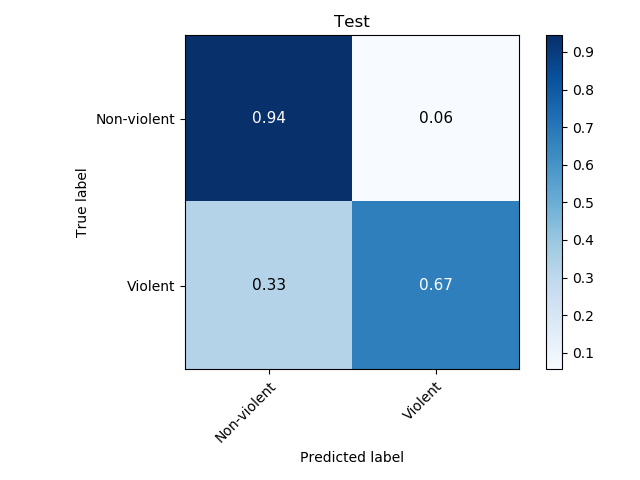
\includegraphics[scale=0.55]{svm-svm-cm-tst}
				\subcaption{SVM multiclass + SVM binary}
			\end{subfigure}
			\vskip\baselineskip
			% 
			\begin{subfigure}[b]{\textwidth}
				\centering
				\captionsetup{justification=centering}
				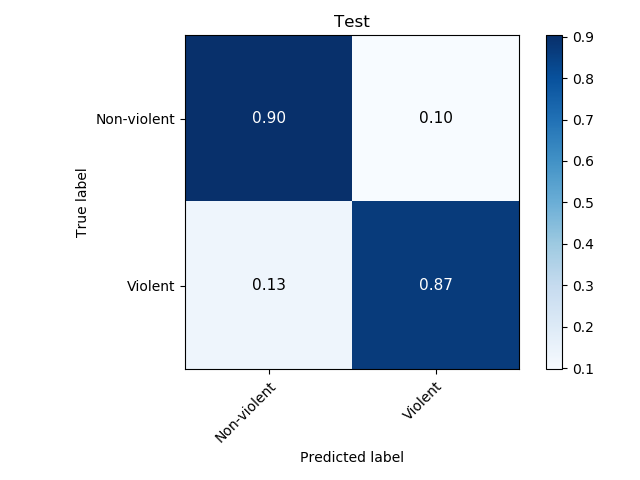
\includegraphics[scale=0.55]{lstm-svm-cm-tst}
				\subcaption{LSTM multiclass + SVM binary}
			\end{subfigure}
			%
			\begin{subfigure}[b]{\textwidth}
				\centering
				\captionsetup{justification=centering}
				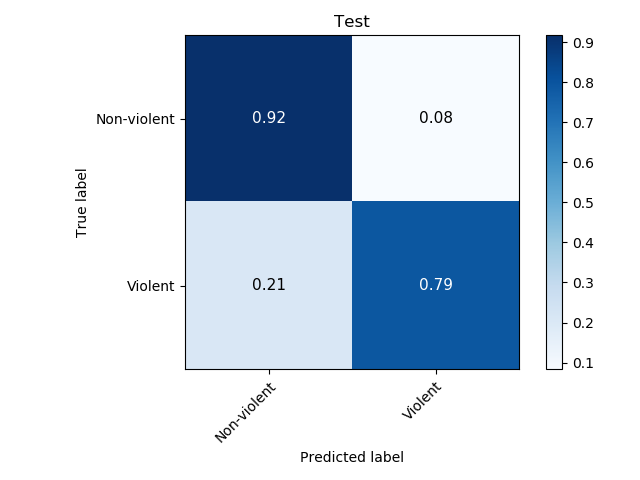
\includegraphics[scale=0.55]{cnn-svm-cm-tst}
				\subcaption{CNN multiclass + SVM binary}
			\end{subfigure}
			\caption{Test confusion matrices}
			\label{fig:mesh46}
		\end{center}
	\end{figure}

	The actual solution of the problem would be this binary classification that allows us to distinguish between non-violent and violent events. The results apparently are really good if we look at the accuracy values, but the interpretability is much more clear when reading the confusion matrices. 
	
	In order to interpret the result for the \acrshort{svm}, we can read the confusion matrix in figure \ref{fig:mesh19} to check how the multiclass classification performed and related to the output obtained from the binary classifier. For this case, certain classes have a wide range of false negatives in non-violent categories, such as \textit{Yell} confused with \textit{Music}. Also, a couple of categories are predicted as \textit{Speech} and some others as \textit{Animal}. If we interpret this errors in a binary context, we can say that the system is taking advantage of the higher a priory of non-violent classes without learning the true distinctions. %they can be resumed by saying that violent labels are predicted as non-violent. 
	This fact is reflected in the only $60\%$ of true positives for the violent label in figure \ref{fig:mesh46} \textit{(a)}. 
	
	In the \acrshort{cnn} approach, the results are numerically smaller but the classification of the violent instances is much better. Almost a $87\%$ of these samples were correctly classified. Again, if we look at figure \ref{fig:mesh34}, some classes are confused within the two different binary labels. A $30\%$ of instances from \textit{Slam} have been wrongly identified as \textit{Speech}. The same happens with \textit{Yell} and \textit{Music} as in the case of \acrshort{svm}. So, these can affect the output of this binary approach and the result of the test confusion matrix. There is also a big mistake in predicting \textit{Slam} for samples that belong to \textit{Breaking}, but this fact does not involve errors in the binary classification.
	
	Finally, the \acrshort{lstm} is the method for which a better result is obtained in this problem. In the confusion matrix in figure \ref{fig:mesh28}, as explained above, we can see some misclassifications but they happen between data of the same type. In a real application this would be a more reasonable result, in order to detect a violent situation without depending too much on the exact event occurred just considering if it is violent or not. This is why the percentage of true positive samples for the violent class is the best for this model with a $82\%$. We can say that this is the best approach from all of our experiments. %the final experiment of the work is the one that involves \acrshort{lstm} as multiclass classifier.
	
	\todo{Esta parte me costó hacerla porque no sabía muy bien por donde tirar. Al final opté por hacer una comparativa de las matrices de confusión mas que de la accuray que es donde mejor se ven los resultados. CPM: bien hecho!}
	
		
	